\documentclass[aspectratio=169,11pt]{beamer}

\usepackage[T1]{fontenc}
\usepackage[utf8]{inputenc}
\usepackage[french]{babel}
\usepackage{lmodern}
\usepackage{booktabs}
\usepackage{tabularx}
\usepackage{graphicx}
\usepackage{appendixnumberbeamer}
\usepackage{tikz}
\usetikzlibrary{positioning,arrows.meta,fit,calc,shapes.geometric,backgrounds,babel}
\usepackage{pgfplots}
\pgfplotsset{compat=1.17}

\usetheme[progressbar=frametitle,numbering=fraction]{metropolis}
\setbeamertemplate{footline}[text line]{\hfill\insertframenumber/\inserttotalframenumber}
\setbeamerfont{footline}{size=\tiny}

\definecolor{acc}{RGB}{235,129,27}
\definecolor{blu}{RGB}{0,95,115}
\definecolor{okg}{RGB}{60,140,80}
\definecolor{bad}{RGB}{190,50,50}
\newcolumntype{L}{>{\raggedright\arraybackslash}X}
\newcommand{\src}[1]{\vfill{\tiny\color{gray}#1}}
\newcommand{\pre}{\textsuperscript{\color{acc}p}}
% Marqueur des diapos et éléments qui sont des propositions (déduit), non des résultats lus.
\newcommand{\prop}{\hfill{\scriptsize\color{acc}\fbox{proposition}}}
% Élément hors corpus (connaissance générale, à vérifier dans le texte de la norme).
\newcommand{\hc}{\textsuperscript{\color{gray}hc}}

\tikzset{
  box/.style={draw=blu, fill=blu!8, rounded corners=3pt, align=center,
              font=\scriptsize, minimum height=8mm, inner sep=4pt},
  hot/.style={box, draw=acc, fill=acc!12},
  ok/.style={box, draw=okg, fill=okg!10},
  ko/.style={box, draw=bad, fill=bad!8},
  risk/.style={font=\tiny, text=bad, align=center},
  arr/.style={-{Stealth[length=2mm]}, thick, gray!70!black},
  darr/.style={arr, dashed},
}

\title{IA embarquée sécuritaire sur FPGA}
\subtitle{État de l'art, verrous et proposition de problématique}
\author{Léonard Rivals}
\institute{Point ARCYS -- ISAE-SUPAERO}
\date{Octobre 2026}

\begin{document}

\maketitle

% ===========================================================================
\section{Le sujet}

\begin{frame}{Sujet et cas d'usage}
  \textbf{Intitulé de travail} : « IA embarquée sécuritaire certifiable sur base de
  technologies FPGA »

  \vspace{0.3em}
  \textbf{Cas d'usage ARCYS}
  \begin{itemize}
    \item détecteur de type YOLO sur flux caméra ;
    \item surveillance de zones industrielles dangereuses où la présence humaine est interdite ;
    \item exigence forte sur les \alert{faux négatifs} (personne non détectée), puis sur
          les faux positifs (arrêts intempestifs) ;
    \item réseau \alert{maîtrisé} : opérations reproduites, sans dépendre de bibliothèques
          « boîte noire ».
  \end{itemize}

  \vspace{0.2em}
  \textbf{Deux volets} : le réseau de neurones embarqué, et la démarche de sûreté /
  certification.\\
  {\small « Sécuritaire » s'entend d'abord au sens \emph{safety} ; la \emph{security} est secondaire.}
\end{frame}

\begin{frame}{Où se loge le risque dans la chaîne}
  \centering
  \begin{tikzpicture}[node distance=4mm and 5mm]
    \node[box] (cam) {Caméra\\scène};
    \node[box, right=of cam] (pre) {Pré-\\traitement};
    \node[hot, right=of pre, minimum width=22mm] (yolo) {YOLO quantifié\\(logique FPGA)};
    \node[box, right=of yolo] (nms) {Décodage\\NMS, suivi};
    \node[box, right=of nms] (dec) {Décision\\zone occupée ?};
    \node[box, right=of dec] (stop) {Arrêt\\machine};
    \draw[arr] (cam) -- (pre); \draw[arr] (pre) -- (yolo); \draw[arr] (yolo) -- (nms); \draw[arr] (nms) -- (dec); \draw[arr] (dec) -- (stop);

    \node[risk, below=3mm of cam] {hors ODD :\\éclairage, poussière,\\occultation};
    \node[risk, below=3mm of yolo] {quantification et\\compilation : écart\\au modèle validé ;\\SEU};
    \node[risk, below=3mm of nms] {code réécrit\\sur l'ARM ;\\débit};
    \node[risk, below=3mm of dec] {seuil :\\faux négatif\\contre arrêt\\intempestif};
    \node[risk, below=3mm of stop] {latence\\pire cas,\\gigue};

    \node[font=\scriptsize, text=blu, above=3mm of yolo] {ce que la littérature FPGA mesure};
    \node[font=\scriptsize, text=blu, above=3mm of dec] {ce qu'une norme de sécurité juge};
  \end{tikzpicture}

  \vspace{0.8em}
  \raggedright\small
  Les articles FPGA évaluent le bloc orange (débit, puissance, mAP). La sûreté se juge sur
  la chaîne entière : une personne manquée, à quel taux par heure, avec quelle preuve.
\end{frame}

\begin{frame}{En bref}
  \begin{enumerate}
    \item \textbf{YOLO sur FPGA existe}, mais la précision est rarement remesurée sur la
          carte, et les pertes après quantification sont parfois fortes et imprévisibles.
    \item \textbf{Les cadres de certification du ML disent quoi prouver}, pas comment le
          faire sur un FPGA ; ils viennent de l'aéronautique et de l'automobile, pas des
          normes de sécurité machine.
    \item \textbf{Les méthodes de sûreté} (fautes, vérification, moniteurs) existent sur
          de petits classifieurs, jamais sur un détecteur implanté sur FPGA.
    \item \textbf{Le croisement est vide} : c'est la place de la thèse.
  \end{enumerate}

  \vspace{0.6em}
  \textbf{Proposition} : un détecteur de personnes sur SoC FPGA dont on \alert{démontre} que
  le circuit fait ce que fait le modèle, et qui \alert{signale} ses situations de doute.
\end{frame}

\begin{frame}{Périmètre de la lecture}
  \begin{columns}[T]
    \begin{column}{0.55\textwidth}
      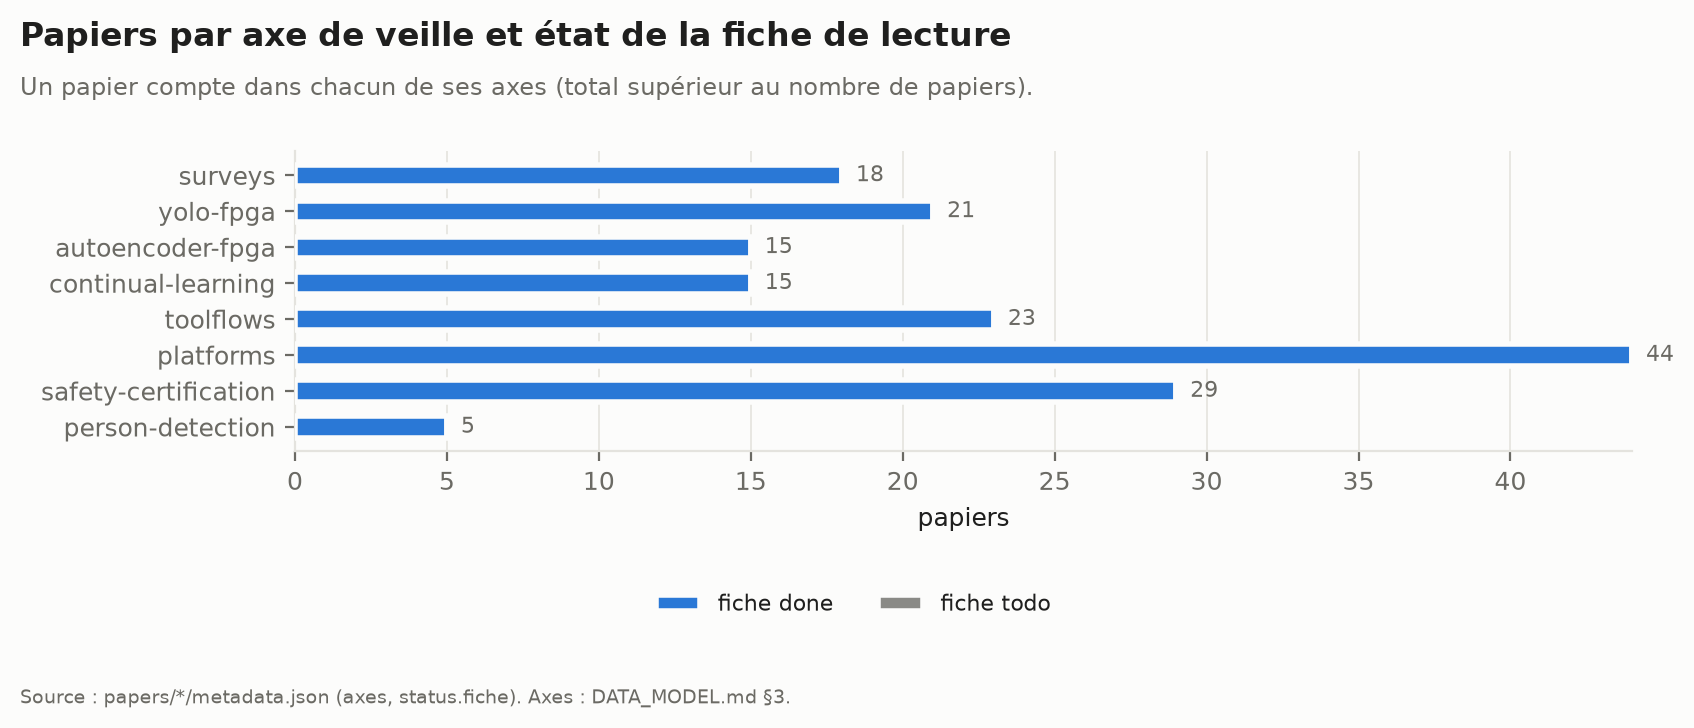
\includegraphics[width=\linewidth]{fig/corpus_axes.png}
    \end{column}
    \begin{column}{0.43\textwidth}
      \footnotesize
      \begin{itemize}
        \item 104 articles, une fiche de lecture critique chacun ;
        \item 306 lignes de benchmarks, liées à leur section source ;
        \item 29 articles sûreté / certification, 5 détection de personnes.
      \end{itemize}
      \textbf{Réserves}
      \begin{itemize}
        \item aucun texte normatif lu directement ;
        \item « absent » = absent des travaux étudiés ;
        \item \pre{} = preprint non relu ; \hc{} = hors corpus, à vérifier.
      \end{itemize}
    \end{column}
  \end{columns}
\end{frame}

% ===========================================================================
\section{YOLO sur FPGA : ce qui existe}

\begin{frame}{Détecteurs YOLO sur FPGA : quelques repères}
  \scriptsize
  \begin{tabularx}{\textwidth}{@{}>{\raggedright\arraybackslash}p{2.4cm} >{\raggedright\arraybackslash}p{3.1cm} >{\raggedright\arraybackslash}p{2.6cm} L@{}}
    \toprule
    Travail & Modèle & Carte / flot & Résultat rapporté \\
    \midrule
    Karki 2026\pre & YOLOv8/11/26 nano INT8 & ZCU104, DPU & 34,05 FPS de bout en bout ;
      mAP@.5:.95 0,66--0,79 (jeu de personnes non publié) ; puissance estimée \\
    Gutierrez 2026\pre & YOLOv3-tiny allégé w2a4 & PYNQ-Z1, FINN & 35,66 FPS ; 2,91 W au
      rail 12 V ; mAP@.5 0,594 (VOC, véhicules) \\
    Fata 2026 & YOLOv3-tiny élagué & KV260, DPU & 24,3 FPS ; « accuracy » au lieu d'une mAP \\
    Montgomerie-C. 2023 & YOLOv5n & ZCU104, SATAY & dataflow, tous les poids on-chip \\
    Zhang 2024 & YOLOv3-tiny & Kintex-7, HLS & 15,2 ms de bout en bout ; NMS en matériel \\
    Schlosser 2023 & YOLOv4 & ZCU104 vs AGX Xavier & Jetson plus rapide
      (22,0 contre 54,42 ms) et plus précis \\
    \bottomrule
  \end{tabularx}

  \vspace{0.3em}
  \small
  Un seul travail mesure un \alert{détecteur de personnes} sur FPGA (Karki 2026, preprint) ;
  les autres portent sur véhicules, VOC, défauts de PCB, drones.
\end{frame}

\begin{frame}{Débit et puissance : un nuage, pas un classement}
  \centering
  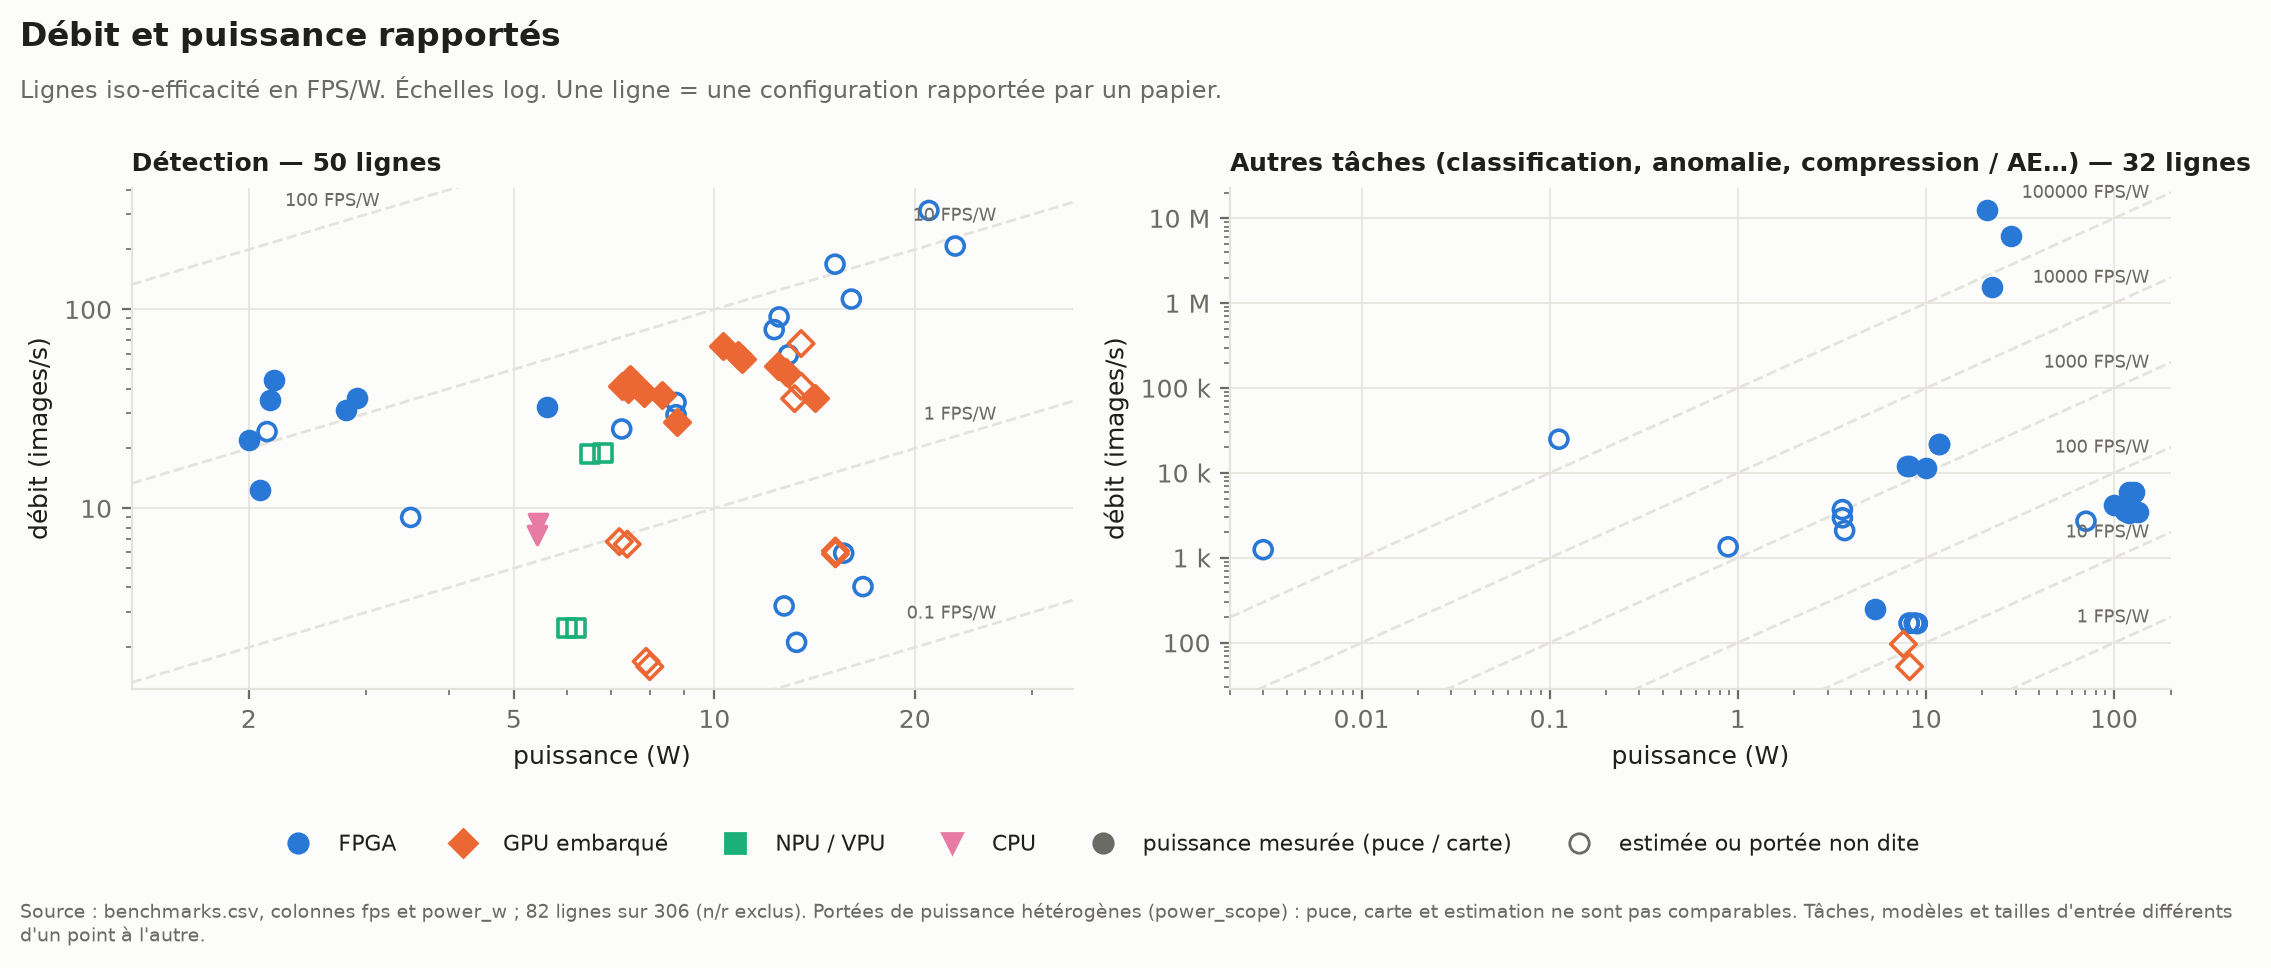
\includegraphics[width=0.86\linewidth]{fig/bench_fps_power.png}

  \raggedright\scriptsize
  Détection : les FPGA occupent la zone 2--25 W, les Jetson 7--15 W, à efficacité voisine
  (1 à 20 FPS/W). Mais la moitié des points FPGA sont des puissances \alert{estimées} ou de
  portée non dite (cercles vides) : le graphique ne permet pas de dire qui gagne.
\end{frame}

\begin{frame}{Deux façons d'implanter : DPU ou dataflow}
  \centering
  \begin{tikzpicture}[node distance=3mm and 6mm]
    \node[box, minimum width=22mm] (m) {Modèle\\PyTorch};
    \node[box, right=of m, yshift=9mm, minimum width=26mm] (vq) {Vitis AI\\quantizer + compilateur};
    \node[ko, right=of vq, minimum width=30mm] (dpu) {DPU : moteur générique\\fermé, jeu d'instructions};
    \node[box, right=of m, yshift=-9mm, minimum width=26mm] (bq) {Brevitas $\to$ QONNX\\$\to$ FINN / hls4ml};
    \node[ok, right=of bq, minimum width=30mm] (df) {Dataflow : un circuit\\par couche, HLS lisible};
    \draw[arr] (m) |- (vq); \draw[arr] (m) |- (bq);
    \draw[arr] (vq) -- (dpu); \draw[arr] (bq) -- (df);
  \end{tikzpicture}

  \vspace{0.5em}
  \scriptsize
  \begin{columns}[T]
    \begin{column}{0.48\textwidth}
      \begin{itemize}
        \item rapide à mettre en œuvre, YOLO récents démontrés ;
        \item impose un modèle modifié (ReLU, attention approchée) : $\approx$\,3 points de
              mAP en plus (Karki 2026\pre) ;
        \item matériel peu inspectable.
      \end{itemize}
    \end{column}
    \begin{column}{0.48\textwidth}
      \begin{itemize}
        \item open source, chaque couche traçable jusqu'au HLS ;
        \item démontré pour un YOLOv3-tiny allégé sur Zynq-7020 (Gutierrez 2026\pre),
              pas pour un YOLO récent sur KV260 ;
        \item limité par la mémoire on-chip ; QAT à $\approx$\,0,006 de mAP du flottant,
              contre $\approx$\,0,17 en PTQ.
      \end{itemize}
    \end{column}
  \end{columns}
\end{frame}

% pgfplots : le « ; » actif de babel french casse la lecture des coordonnées
{\shorthandoff{;}
\begin{frame}{La précision après quantification est rarement vérifiée sur la cible}
  \begin{columns}[c]
    \begin{column}{0.5\textwidth}
      \begin{tikzpicture}
        \begin{axis}[
          ybar, bar width=7pt, width=\linewidth, height=5.2cm,
          ymin=0, ymax=1.05, ylabel={\scriptsize mAP@.5:.95},
          symbolic x coords={a, b, c},
          xticklabels={v8n VOC, v8n KITTI, v11n CCTV},
          xtick=data, tick label style={font=\scriptsize},
          legend style={font=\tiny, at={(0.5,1.02)}, anchor=south, legend columns=2},
          /pgf/number format/use comma,
          nodes near coords, nodes near coords style={font=\tiny},
          enlarge x limits=0.25]
          \addplot[fill=blu!60, draw=blu] coordinates {(a,0.60) (b,0.64) (c,0.75)};
          \addplot[fill=acc!70, draw=acc] coordinates {(a,0.45) (b,0.34) (c,0.71)};
          \legend{CPU flottant, FPGA INT8 (DPU)}
        \end{axis}
      \end{tikzpicture}

      {\tiny\color{gray} Karki 2026\pre, Table II.}
    \end{column}
    \begin{column}{0.48\textwidth}
      \small
      \begin{itemize}
        \item écarts jugés \alert{imprévisibles} d'un modèle à l'autre ;
        \item YOLOv4, Vitis AI : $-2{,}2$ points à la quantification, puis encore à la
              compilation (Schlosser 2023) ;
        \item TensorRT INT8 : $-6{,}4$ à $-12{,}3$ points, conclu « sans perte significative »
              (Rey 2025).
      \end{itemize}
    \end{column}
  \end{columns}

  \vspace{0.4em}
  \textbf{Conséquence} : une propriété validée sur le modèle entraîné n'est pas garantie sur
  le circuit. Problème de performance \emph{et} de certification (objectif EASA IMP-06).
\end{frame}}

\begin{frame}{Les mesures publiées sont difficilement comparables}
  \small
  Recompte de la base : 216 lignes mesurées sur FPGA, 44 articles.
  \begin{itemize}
    \item \textbf{puissance} : 115 lignes en ont une, 47 seulement mesurée (10 articles) ;
          une seule paire puce / carte sur une même FPGA (7,8 W Vivado contre 12,3 W au
          wattmètre, Zhang 2024) ;
    \item \textbf{précision} : 87 lignes de détection, 14 libellés de précision différents ;
          6 lignes seulement mesurées sur la carte de façon établie (Schlosser, Karki\pre) ;
    \item \textbf{latence} : toujours en moyenne ; aucun pire cas, p99 ni gigue de bout en bout ;
    \item \textbf{comparaisons flatteuses} : GOPS/DSP face à un autre modèle, « 70x » face
          à un GPU qui fait 44,6 FPS contre 24,3 sur la KV260 (Fata 2026) ;
    \item aucun bitstream publié, code rarement disponible.
  \end{itemize}

  \vspace{0.3em}
  Cadre de mesure le plus complet : Schlosser 2023 (mAP sur la cible, puissance de carte au
  multimètre, repos soustrait), mais un seul modèle et sans pire cas.
\end{frame}

% ===========================================================================
\section{Cadres de certification du ML}

\begin{frame}{Le cycle en W et le principe Doer / Checker (EASA CoDANN)}
  \centering
  \begin{tikzpicture}[scale=0.72, transform shape, node distance=2mm and 3mm, every node/.style={font=\tiny}]
    \node[box] (req) {Exigences\\système};
    \node[box, below right=4mm and 0mm of req] (dat) {Gestion des\\données};
    \node[box, below right=4mm and 0mm of dat] (lrn) {Apprentissage};
    \node[box, above right=4mm and 0mm of lrn] (lv) {Vérification\\du modèle appris};
    \node[box, below right=4mm and 0mm of lv, draw=acc, fill=acc!12] (imp) {Implémentation\\(quantif., cible)};
    \node[box, above right=4mm and 0mm of imp] (iv) {Vérification du\\modèle d'inférence};
    \node[box, above right=4mm and 0mm of iv] (sv) {Vérification\\système};
    \draw[arr] (req) -- (dat); \draw[arr] (dat) -- (lrn); \draw[arr] (lrn) -- (lv);
    \draw[arr] (lv) -- (imp); \draw[arr] (imp) -- (iv); \draw[arr] (iv) -- (sv);
    \node[below=1mm of imp, text=bad, align=center] {FPGA « will not be addressed »\\(CoDANN I, §4.2.3)};
  \end{tikzpicture}
  \hspace{3mm}
  \begin{tikzpicture}[scale=0.72, transform shape, node distance=4mm, every node/.style={font=\scriptsize}]
    \node[box, minimum width=22mm] (in) {Entrée};
    \node[hot, below left=5mm and -6mm of in, minimum width=20mm] (doer) {Doer\\réseau};
    \node[ok, below right=5mm and -6mm of in, minimum width=20mm] (chk) {Checker\\discrim. OOD};
    \node[box, below=16mm of in, minimum width=22mm] (out) {Sortie ou repli};
    \draw[arr] (in) -- (doer); \draw[arr] (in) -- (chk);
    \draw[arr] (doer) -- (out); \draw[arr] (chk) -- (out);
  \end{tikzpicture}

  \vspace{0.3em}
  \raggedright\footnotesize
  CoDANN (EASA, 2020) : cycle en W (§6.1), fonction et moniteur séparés (§6.6). Bornes de
  généralisation inutilisables sur de gros réseaux : la garantie repose sur un
  échantillonnage i.i.d.\ du domaine (§5.3.5).
\end{frame}

\begin{frame}{EASA Concept Paper (Issue 02, 2024) : les objectifs qui nous touchent}
  \footnotesize
  \begin{tabularx}{\textwidth}{@{}p{2.6cm} L p{3.6cm}@{}}
    \toprule
    Objectif & Ce qu'il demande & Conséquence pour la thèse \\
    \midrule
    MOC LM-02 & modèle gelé à l'approbation ; apprentissage en ligne non accepté &
      tension avec l'apprentissage continu \\
    LM-06 & la quantification qui change le comportement relève de l'apprentissage &
      la QAT fait partie de la preuve \\
    MOC IMP-04-2 & en implémentation, seules les optimisations sans effet sur le
      comportement sont admises & compilation DPU à justifier \\
    MOC IMP-05 & FPGA et ASIC : guides existants (AMC 20-152A) ; GPU : guides à créer &
      \alert{avantage FPGA} \\
    IMP-06 & préservation des propriétés après conversion ; méthodes formelles
      « expected to be necessary » & \alert{verrou 1} \\
    EXP-04 à 07, SRM-02 & surveiller ODD, distribution et confiance ; repli sur un système
      classique & \alert{verrou 3} \\
    \bottomrule
  \end{tabularx}

  \vspace{0.4em}
  \small
  Document non contraignant (moyens de conformité « anticipated »). Seul cas de vision :
  Visual Landing System, sur GPU COTS non certifié (§F.2.1.3.3) ; rien sur les SEU.
\end{frame}

\begin{frame}{CoDANN II (2024) : du modèle entraîné au modèle déployé}
  \begin{columns}[T]
    \begin{column}{0.5\textwidth}
      \small
      \textbf{Trois niveaux d'équivalence} (§3.6.1)
      \begin{itemize}
        \item \emph{ponctuelle} : même sortie, entrée par entrée ;
        \item \emph{proximité ponctuelle} : écart borné, entrée par entrée ;
        \item \emph{en moyenne} : mêmes performances statistiques.
      \end{itemize}
      Borne de généralisation évaluée \alert{sur le modèle transformé}, dans
      l'environnement d'inférence (§3.7.3) ; outils qualifiés selon DO-178C §12.2 (§3.7.1).
    \end{column}
    \begin{column}{0.48\textwidth}
      \small
      \textbf{Moniteur et matériel}
      \begin{itemize}
        \item le moniteur hors distribution reçoit le même niveau d'assurance que la
              fonction (§5.2.2) ;
        \item FPGA plus visible que le GPU (pilotes, microcode, ordonnancement
              propriétaires) (§3.2.2, annexe B).
      \end{itemize}
      {\scriptsize\color{gray} Argument de l'entreprise Daedalean, sans mesure ; sections
      sûreté et DAL retirées de la version publique.}
    \end{column}
  \end{columns}

  \vspace{0.2em}
  \textbf{Lecture pour le FPGA} : un flot dataflow en virgule fixe vise l'équivalence
  \emph{ponctuelle} (bit à bit), là où le GPU ne peut viser que la proximité.
  {\scriptsize\color{acc}(déduit)}
\end{frame}

\begin{frame}{Guides académiques : AMLAS, DEEL, Ashmore, Salay}
  \small
  \begin{itemize}
    \item \textbf{AMLAS} (Hawkins 2021\pre) : six étapes, chacune close par un argument GSN ;
          exemple d'exigence « identifier toute personne présente avec une précision d'au
          moins 0,93 » (Stage 2, Ex. 7) ; matériel vu seulement à l'intégration (Stage 6).
    \item \textbf{DEEL} (Delseny 2021\pre) : sept défis ; perte \alert{asymétrique} (piéton
          manqué catastrophique, fausse détection « major », §4.2.4.2) ; conversion d'un taux
          d'erreur par image en taux par heure (§4.2.4.4) ; implémentation hors périmètre.
    \item \textbf{Ashmore 2019\pre} : tester sur la cible, car la représentation numérique
          change entre étapes (§7.4.1) ; surveiller les internes du modèle contre les SEU
          (§7.2.2).
    \item \textbf{Salay 2017\pre} (ISO 26262) : « reconnaître un piéton » est peut-être
          inspécifiable ; pour les ASIL élevés, reconnaisseurs redondants entraînés sur des
          modèles et données différents (§III-C).
  \end{itemize}

  \vspace{0.3em}
  Tous partent de l'aéronautique ou de l'automobile.
\end{frame}

\begin{frame}{Cas de référence : Certified ML Object Detection for Surveillance Missions}
  \small
  Belcaid et al., ERTS 2024 : détection de drones intrus,
  démarche ED-324 / ARP 6983 appliquée en partie.

  \begin{columns}[T]
    \begin{column}{0.5\textwidth}
      \textbf{Ce qui est fait}
      \begin{itemize}
        \item ODD système, puis ODD du composant ML (taille, position, luminosité) ;
        \item biais de position du jeu corrigé, augmentation ;
        \item YOLOv3-tiny, image 1920$\times$1080 découpée en tuiles ;
        \item GEMM réécrit en CUDA, sans cuBLAS.
      \end{itemize}
    \end{column}
    \begin{column}{0.5\textwidth}
      \textbf{Limites}
      \begin{itemize}
        \item cible Jetson AGX Xavier : traçabilité arrêtée aux pilotes NVIDIA ;
        \item exigences : détection $>$ 80\,\%, latence $<$ 50 ms ; 15 ms obtenues en FP16,
              tuile ou image non précisé ;
        \item aucune métrique de détection publiée ;
        \item ni vérification, ni moniteur hors ODD.
      \end{itemize}
    \end{column}
  \end{columns}

  \vspace{0.5em}
  \alert{Transposable} : démarche ODD et données. \alert{À faire} : la même chose avec un
  accélérateur dont le RTL / HLS est inspectable.
\end{frame}

% ===========================================================================
\section{Normes industrielles}

\begin{frame}{Ce que le corpus dit des normes de sécurité machine}
  \begin{itemize}
    \item aucune fiche ne traite IEC 61508, ISO 13849, IEC 62061 ou ISO/IEC TR 5469 pour
          elles-mêmes ;
    \item IEC 61508 citée comme contexte (Li 2017, §1) ; cible $<$ 10 FIT tirée
          d'ISO 26262, reprise pour l'ASIL D (Rech 2024, §III-C) ;
    \item Halme 2018 (vision pour la collaboration humain-robot) : s'appuie sur ISO 10218-1/2
          et ISO/TS 15066 ; sur 15 méthodes de vision, \alert{une seule commerciale et
          certifiée} (SafetyEYE, Table 1) ;
    \item difficultés listées par Halme : occultations, sensibilité des caméras 2D à la
          lumière et à la poussière, latence de perception non traitée (§4).
  \end{itemize}

  \vspace{0.6em}
  \textbf{Constat} : les cadres ML existants (EASA, AMLAS, DEEL) ne sont mis en
  correspondance avec aucune norme industrielle. C'est un travail à faire, et une
  question pour ARCYS : \alert{quelle norme vise le produit ?}
\end{frame}

\begin{frame}{Paysage normatif à positionner}
  \scriptsize
  \begin{tabularx}{\textwidth}{@{}p{3.3cm} p{3.4cm} p{2.2cm} L@{}}
    \toprule
    Texte & Domaine & Niveau d'intégrité & Statut vis-à-vis du ML \\
    \midrule
    IEC 61508\hc & sécurité fonctionnelle générique & SIL 1--4 (PFH) & pas de ML ; base
      des normes sectorielles \\
    IEC 62061\hc & machines (commande électrique) & SIL 1--3 & dérivée d'IEC 61508 \\
    ISO 13849-1\hc & machines (parties de commande) & PL a--e & architectures par
      catégories, pas de ML \\
    IEC 61496 / TS 61496-4-3\hc & équipements de protection électrosensibles, vision &
      types 2--4 & dispositifs de protection par caméra ; pas de réseau appris \\
    ISO/IEC TR 5469 (2024)\hc & IA et sécurité fonctionnelle & --- & rapport technique :
      classes d'usage de l'IA, mesures de maîtrise \\
    ED-324 / ARP 6983 & aéronautique & DAL & processus ML, en cours ; appliqué par
      Belcaid 2024 \\
    \bottomrule
  \end{tabularx}

  \vspace{0.3em}
  \footnotesize
  \hc{} hors corpus : rappels de connaissance générale, à vérifier dans les textes.
  \textbf{Action} : lire TR 5469 et la série IEC 61496 en priorité ; ce sont les plus proches
  d'une « caméra qui protège des personnes ».
\end{frame}

% pgfplots : le « ; » actif de babel french casse la lecture des coordonnées
{\shorthandoff{;}
\begin{frame}{L'ordre de grandeur à combler}
  \begin{columns}[c]
    \begin{column}{0.5\textwidth}
      \begin{tikzpicture}
        \begin{axis}[
          xbar, scale only axis, width=0.62\linewidth, height=3.4cm, xmode=log,
          xmin=1e-9, xmax=1, log origin x=infty,
          xlabel={\scriptsize défaillances dangereuses par heure},
          symbolic y coords={s3, s2, s1, det},
          ytick={s3, s2, s1, det},
          yticklabels={SIL 3 / PL e, SIL 2 / PL d, SIL 1 / PL c, Détecteur seul}, tick label style={font=\scriptsize}, bar width=8pt,
          enlarge y limits=0.2, bar shift=0pt]
          \addplot[fill=acc!70, draw=acc] coordinates {(6e-2,det)};
          \addplot[fill=blu!50, draw=blu] coordinates {(1e-5,s1) (1e-6,s2) (1e-7,s3)};
        \end{axis}
      \end{tikzpicture}

      {\tiny\color{gray} Bornes hautes des niveaux : hors corpus\hc, à vérifier.}
    \end{column}
    \begin{column}{0.48\textwidth}
      \small
      \textbf{Calcul de DEEL} (§4.2.4.4) : un obstacle par minute et $10^{-3}$ d'erreur par
      image donnent $6\cdot10^{-2}$ défaillance par heure.

      \vspace{0.4em}
      Écart à un SIL 2 : \alert{4 à 5 ordres de grandeur}. Aucun réseau ne les gagne seul.
      Ils doivent venir de l'architecture : moniteur, redondance, vote temporel sur plusieurs
      images, repli. {\scriptsize\color{acc}(déduit)}
    \end{column}
  \end{columns}

  \vspace{0.4em}
  \small
  D'où l'intérêt de raisonner sur la \alert{chaîne} (détecteur + moniteur + suivi), et de
  mesurer ce que chaque élément gagne.
\end{frame}}

% ===========================================================================
\section{Les verrous}

\begin{frame}{Six verrous, vus d'ensemble}
  \footnotesize
  \begin{tabularx}{\textwidth}{@{}p{3.6cm} L L@{}}
    \toprule
    Verrou & Ce qui existe & Ce qui manque \\
    \midrule
    1. Circuit = modèle ? & code traçable FP32 sur CPU (ACETONE) & aucune preuve
      modèle quantifié $\to$ bitstream \\
    2. Vérification formelle & réseaux denses $\leq$ 52\,650 paramètres & un détecteur
      convolutif \\
    3. Moniteur d'exécution & MSP, patrons, boîtes, conforme ; sur CPU / GPU & implanté sur
      FPGA, coût mesuré \\
    4. Fautes matérielles (SEU) & classifieurs de 19 poids à VGG-16 & un YOLO, un DPU,
      les BRAM \\
    5. Erreur dangereuse & critère par boîtes (Rech 2024) & lien taux d'erreur $\to$ SIL / PL \\
    6. Déterminisme & argument CoDANN II, sans mesure & pire cas et gigue mesurés \\
    \bottomrule
  \end{tabularx}

  \vspace{0.5em}
  \small
  Les verrous 1 et 3 sont les plus proches du cas ARCYS et du savoir-faire de l'équipe
  d'Arnaud (code certifiable pour FPGA) ; le 4 est secondaire au sol.
\end{frame}

\begin{frame}{Verrou 1 : prouver que le circuit fait ce que fait le modèle}
  \centering
  \begin{tikzpicture}[node distance=3mm and 4mm]
    \node[box] (pt) {Modèle\\flottant};
    \node[box, right=of pt] (q) {Modèle\\quantifié (QAT)};
    \node[box, right=of q] (onnx) {QONNX\\graphe};
    \node[box, right=of onnx] (hls) {C++ HLS\\par couche};
    \node[box, right=of hls] (rtl) {RTL};
    \node[hot, right=of rtl] (bit) {Bitstream\\sur carte};
    \draw[arr] (pt) -- (q); \draw[arr] (q) -- (onnx); \draw[arr] (onnx) -- (hls); \draw[arr] (hls) -- (rtl); \draw[arr] (rtl) -- (bit);
    \node[risk, below=2mm of q] {validé ici\\(LM-06)};
    \node[risk, below=2mm of onnx] {arrondis,\\saturations non\\garantis entre outils};
    \node[risk, below=2mm of hls] {outil non\\qualifié (TQL)};
    \node[risk, below=2mm of bit] {jamais\\remesuré};
    \draw[darr, okg] (q.north) to[bend left=18] node[above, font=\tiny, text=okg]
      {piste : équivalence bit à bit, couche par couche} (bit.north);
  \end{tikzpicture}

  \vspace{0.3em}
  \raggedright\footnotesize
  \begin{itemize}
    \item CoDANN I renvoie l'implémentation à plus tard ; IMP-06 la demande sans moyen
          de conformité ; la qualification d'outil (DO-178C §12.2) n'a jamais été appliquée à
          FINN ni à Vitis AI ;
    \item ACETONE (de Albuquerque Silva 2022) : C traçable, écart $\approx 10^{-6}$ en FP32,
          sémantique \emph{testée}, non prouvée ; WCET hors de portée pour AlexNet.
  \end{itemize}
  \textbf{Piste} : en virgule fixe, l'équivalence ponctuelle est atteignable ; la vérifier par
  tests exhaustifs ou preuve, couche par couche, sur un flot FINN.
\end{frame}

% pgfplots : le « ; » actif de babel french casse la lecture des coordonnées
{\shorthandoff{;}
\begin{frame}{Verrou 2 : la vérification formelle ne passe pas à l'échelle}
  \begin{columns}[c]
    \begin{column}{0.5\textwidth}
      \begin{tikzpicture}
        \begin{axis}[
          xbar, scale only axis, width=0.45\linewidth, height=3.8cm, xmode=log, xmin=10, xmax=1e7,
          log origin x=infty, ytick={yolo, approx, qnn, acas},
          xlabel={\scriptsize taille (échelle log)},
          symbolic y coords={yolo, approx, qnn, acas},
          yticklabels={YOLOv8n (param.)\hc, Bornes approchées (neur.), QNN bit-exact (param.), ACAS Xu (ReLU)},
          tick label style={font=\tiny}, bar width=7pt, enlarge y limits=0.18, bar shift=0pt]
          \addplot[fill=blu!50, draw=blu] coordinates {(300,acas) (52650,qnn) (10000,approx)};
          \addplot[fill=acc!70, draw=acc] coordinates {(3.2e6,yolo)};
        \end{axis}
      \end{tikzpicture}
    \end{column}
    \begin{column}{0.48\textwidth}
      \scriptsize
      \begin{itemize}
        \item Reluplex (Katz 2017\pre) : 45 réseaux de 300 ReLU ; $\varphi_1$ prouvée sur
              41 en 394\,517 s, 4 timeouts ;
        \item BNN en SAT (Narodytska 2017\pre) : robustesse certifiée pour au plus 21 images
              sur 200 ; permet aussi l'équivalence de deux réseaux ;
        \item QNN bit-exact (Henzinger 2021) : PSPACE-difficile ; réseau dense de 52\,650
              paramètres ;
        \item méthodes à bornes approchées : au plus $\approx$\,10\,000 neurones cachés
              (Huang 2018\pre, §4.2--4.3).
      \end{itemize}
    \end{column}
  \end{columns}

  \vspace{0.4em}
  \small
  Unités différentes : l'ordre de grandeur seul compte. Propriétés vérifiées : robustesse
  locale, sans lien avec un danger. \textbf{Piste} : vérifier des \alert{composants} (moniteur,
  tête, NMS) et l'équivalence réseau quantifié / circuit, compléter par des garanties
  statistiques.
\end{frame}}

\begin{frame}{Verrou 3 : un détecteur qui signale son incertitude}
  \scriptsize
  \begin{tabularx}{\textwidth}{@{}p{3.3cm} p{2cm} L@{}}
    \toprule
    Moniteur & Testé sur & Résultat et limite \\
    \midrule
    Score softmax max. (Hendrycks 2017) & classifieur & AUROC 95 CIFAR / SUN, 61 presque
      en distribution \\
    Patrons d'activation (Cheng 2018\pre) & GTSRB & muet 95,42\,\% du temps ; couche
      surveillée limitée à $\approx$\,200 neurones \\
    Boîtes d'abstraction (Henzinger 2020) & classifieur & $<$ 1 ms par entrée ; mémoire
      indépendante de la taille du jeu \\
    SafeML (Aslansefat 2020\pre) & cas jouet & estime 0,772 pour une vraie exactitude de
      0,508 : erreur dans le sens dangereux \\
    Gaussian YOLOv3 (Choi 2019) & KITTI, GPU & +0,04\,\% de FLOPs ; $-41{,}4$\,\% de faux
      positifs \\
    Prédiction conforme (Andéol 2023\pre) & YOLOv5m, rail & couverture 0,92--1,00 pour
      0,9 visé ; \alert{ne couvre pas les faux négatifs} \\
    \bottomrule
  \end{tabularx}

  \vspace{0.5em}
  \small
  Demandés par l'EASA (EXP-04 à 07), \alert{jamais implantés sur FPGA}. Plusieurs se réduisent
  à des comparaisons et additions : a priori peu coûteux en logique {\scriptsize\color{acc}(déduit)}.
  \textbf{Piste} : moniteur à côté d'un YOLO sur KV260 ; ressources, latence ajoutée, erreurs
  détectées à fausse alarme fixée.
\end{frame}

\begin{frame}{Verrou 4 : fiabilité matérielle (SEU) d'un détecteur}
  \small
  \begin{itemize}
    \item \textbf{Libano 2019} (Zynq, ZU9EG, neutrons) : TMR de la seule couche la plus
          vulnérable $\to$ $-64{,}2$\,\% d'erreurs, contre $-85{,}1$\,\% en TMR complet ; sur un CNN
          MNIST, $\approx$\,40\,\% des fautes masquées pour +8\,\% de ressources ; BRAM exclues ;
    \item \textbf{Libano 2020} : binariser baisse la section efficace de 39\,\%, mais les
          erreurs critiques passent de 26 à 38\,\% ; au sol, l'inexactitude du modèle domine ;
    \item \textbf{Gambardella 2019} (FINN, ZCU104) : un canal bloqué coûte jusqu'à 10,8 points ;
          réplication sélective : +49,87\,\% de MAC pour 2\,\% de chute tolérée, contre +200\,\% ;
    \item \textbf{Li 2017} : 7,19\,\% de corruptions silencieuses en virgule fixe contre
          0,38\,\% en flottant ; bornes d'activation par couche : FIT d'Eyeriss 8,55 $\to$ 0,35 ;
    \item \textbf{Rech 2024} : cohérence temporelle entre images $\approx$\,70\,\% des erreurs
          critiques détectées.
  \end{itemize}

  \vspace{0.3em}
  Toujours des classifieurs ; aucune injection dans un DPU ni sur un YOLO.
  {\scriptsize Volet probablement secondaire pour le cas ARCYS au sol.}
\end{frame}

\begin{frame}{Verrou 5 : qu'est-ce qu'une erreur dangereuse ?}
  \begin{itemize}
    \item critère d'erreur des études de fiabilité : celui d'un classifieur (changement de
          classe) ;
    \item Rech 2024 : erreur critique de détection par seuil de Jaccard sur les boîtes,
          sans lien avec SIL ou PL ;
    \item aucun papier ne traduit un taux d'erreur ou un FIT en SIL / PL ;
    \item asymétrie faux négatif / fausse alarme posée par EASA et DEEL, sans métrique pour la
          détection de personnes.
  \end{itemize}

  \vspace{0.5em}
  \textbf{À définir} \prop
  \begin{itemize}
    \item événement redouté : « personne présente dans la zone, non signalée pendant $N$
          images consécutives, à distance $\leq d$ » ;
    \item taux de défaillance dangereuse par heure qui combine erreurs du modèle, fautes
          matérielles et couverture du moniteur.
  \end{itemize}
\end{frame}

\begin{frame}{Verrou 6 : le déterminisme du FPGA reste à mesurer}
  \begin{itemize}
    \item CoDANN II plaide pour le FPGA : pas de microcode secret, pas de DVFS, pas de
          multicœur partagé ; mais sans mesure ;
    \item côté GPU : traçabilité bloquée aux pilotes (Belcaid 2024) ;
    \item côté FPGA : latences publiées en moyenne, latence variable selon la vidéo
          (Fata 2026, Fig. 14) ; post-traitement sur l'ARM souvent limitant ;
    \item aucun pire cas, p99 ni gigue de bout en bout publié.
  \end{itemize}

  \vspace{0.6em}
  \textbf{Question candidate} : le FPGA rend-il la borne de latence d'un détecteur
  \alert{démontrable} ? Comparer DPU, FINN et Jetson sur le même YOLO, sur $10^5$ images,
  pré- et post-traitement compris.
\end{frame}

\begin{frame}{Apprentissage continu contre certification}
  \begin{itemize}
    \item EASA : l'apprentissage en ligne « will not be accepted by EASA at this stage »
          (MOC LM-02) ;
    \item CoDANN, AMLAS, DEEL : système gelé, apprentissage hors ligne ;
    \item côté apprentissage continu embarqué : ni non-régression, ni versionnage, ni retour
          arrière.
  \end{itemize}

  \vspace{0.6em}
  \textbf{Piste} \prop\\
  Backbone gelé et certifié, petite tête adaptée sous contraintes (SLDA, OS-ELM), test de
  non-régression embarqué avant activation, retour arrière. \\
  {\small Utile si la thèse doit garder un lien avec l'adaptation en service ; sinon,
  perspective.}
\end{frame}

% ===========================================================================
\section{Détection de personnes}

\begin{frame}{Données et métriques pour la détection de personnes}
  \begin{itemize}
    \item CrowdHuman : 22,64 personnes par image ; taux d'échec moyen 50,42 sur le corps
          entier contre 10,08 sur Caltech ; images du web (Shao 2018\pre) ;
    \item \alert{aucun jeu industriel} : EPI, machines, éclairage dégradé, poussière ;
    \item métriques publiées : mAP ou taux d'erreur moyennés ; aucun rappel à taux de fausse
          alarme fixé, par distance ou par occultation ;
    \item le cas complet le plus proche (Belcaid 2024) ne publie pas de métrique.
  \end{itemize}

  \vspace{0.6em}
  \textbf{Piste} : YOLO nano de personnes, opérateurs compatibles DPU et FINN, entraîné sur
  CrowdHuman ; \alert{rappel à 0,1 FPPI} mesuré sur KV260, en flottant et en INT8. Puis un
  ODD d'exemple et des images de site fournies par ARCYS.
\end{frame}

\begin{frame}{Robustesse et chaîne détection, suivi, identification}
  \textbf{Robustesse adverse}
  \begin{itemize}
    \item un patch imprimé fait tomber le rappel de YOLOv2 de 100 à 26,46\,\% (Thys 2019\pre) ;
    \item effet de la quantification et du FPGA sur cette vulnérabilité : non étudié.
  \end{itemize}

  \vspace{0.5em}
  \textbf{Suivi et identification}
  \begin{itemize}
    \item suivi sur l'ARM : le débit peut tomber de 195 à 24 FPS ;
    \item aucune chaîne détection + suivi + Re-ID complète sur SoC FPGA ;
    \item le suivi peut servir la sûreté : vote temporel, persistance d'une personne
          (rejoint les $\approx$\,70\,\% d'erreurs détectées par cohérence temporelle, Rech 2024).
  \end{itemize}
\end{frame}

% ===========================================================================
\section{Synthèse}

\begin{frame}{Le croisement central est vide}
  \centering
  \begin{tikzpicture}[node distance=6mm and 10mm]
    \node[box, minimum width=48mm, minimum height=26mm] (yolo)
      {\textbf{YOLO sur FPGA}\\[2pt]accélérateurs, DPU, FINN\\débit, puissance\\[2pt]
       \textit{sans sûreté}};
    \node[box, minimum width=48mm, minimum height=26mm, right=34mm of yolo] (safe)
      {\textbf{Sûreté du ML}\\[2pt]fiabilité, vérification,\\moniteurs, certification\\[2pt]
       \textit{sur classifieurs ou GPU}};
    \path (yolo) -- (safe) node[midway, hot, minimum width=28mm, minimum height=16mm] (gap)
      {\textbf{Thèse}\\détecteur de personnes\\quantifié, sûr, sur FPGA};
    \draw[arr] (yolo) -- (gap);
    \draw[arr] (safe) -- (gap);
  \end{tikzpicture}

  \vspace{0.8em}
  \raggedright
  Dans les travaux étudiés, aucun détecteur quantifié sur FPGA n'est soumis à la fois à
  une mesure de précision sur cible, à un moniteur d'exécution et à une analyse de fiabilité.
  Les deux moitiés existent, séparément.
\end{frame}

\begin{frame}{Ce qu'il manquerait, au minimum}
  \begin{enumerate}
    \item une correspondance entre objectifs EASA / AMLAS et normes industrielles ;
    \item une métrique de criticité propre à la détection de personnes, reliée à un taux de
          défaillance par heure, puis à un SIL ou un PL ;
    \item une preuve, ou au moins une borne mesurée, de l'écart entre le modèle de référence
          et le circuit déployé ;
    \item un moniteur d'exécution implanté sur la même puce, au coût et à la latence mesurés ;
    \item une campagne d'injection de fautes sur un YOLO quantifié, BRAM comprises ;
    \item un jeu de personnes en zone industrielle sur lequel évaluer le tout.
  \end{enumerate}

  \vspace{0.4em}
  \small
  Une thèse ne couvre pas les six : il faut choisir. Les points 2, 3 et 4 forment un tout
  cohérent et démontrable sur une carte. {\scriptsize\color{acc}(déduit)}
\end{frame}

% ===========================================================================
\section{Problématique et plan}

\begin{frame}{Proposition de problématique \prop}
  \begin{block}{Problématique principale}
    Comment \alert{démontrer} qu'un détecteur de personnes quantifié, implanté sur SoC FPGA,
    conserve sur la carte les propriétés validées sur le modèle, et \alert{signale à
    l'exécution} les situations où il risque de manquer une personne, à un coût matériel
    et une latence bornés ?
  \end{block}

  \vspace{0.3em}
  \small
  \begin{columns}[T]
    \begin{column}{0.48\textwidth}
      \textbf{Variante A -- chaîne certifiable}\\
      contraintes de conception (opérations, virgule fixe, architecture) pour une génération
      de code et une équivalence bit à bit ; proche des thèses encadrées par Arnaud.
    \end{column}
    \begin{column}{0.48\textwidth}
      \textbf{Variante B -- moniteur embarqué}\\
      détecteur qui estime son incertitude sur FPGA ; couverture des faux négatifs, coût
      matériel, contribution au taux de défaillance par heure.
    \end{column}
  \end{columns}

  \vspace{0.4em}
  Objet expérimental commun : un YOLO nano de personnes sur KV260.
\end{frame}

\begin{frame}{Architecture cible \prop}
  \centering
  \begin{tikzpicture}[node distance=4mm and 6mm]
    \node[box] (cam) {Caméra};
    \node[box, right=of cam] (pre) {Pré-\\traitement};
    \node[hot, right=10mm of pre, yshift=7mm, minimum width=28mm] (det) {Détecteur YOLO\\dataflow INT8};
    \node[ok, right=10mm of pre, yshift=-7mm, minimum width=28mm] (mon) {Moniteur\\incertitude / OOD};
    \node[box, right=10mm of det, yshift=-7mm, minimum width=24mm] (post) {NMS, suivi,\\vote temporel};
    \node[box, right=of post] (dec) {Décision\\sûre / repli};
    \begin{scope}[on background layer]
      \node[draw=gray, dashed, rounded corners, fit=(det)(mon), inner sep=3mm] (pl) {};
    \end{scope}
    \node[font=\tiny, text=gray, above=0mm of pl] {logique programmable (PL)};
    \draw[arr] (cam) -- (pre); \draw[arr] (pre) -- (det.west); \draw[arr] (pre) -- (mon.west);
    \draw[arr] (det.east) -- (post); \draw[arr] (mon.east) -- (post); \draw[arr] (post) -- (dec);

    \node[box, below=12mm of mon, xshift=-14mm, minimum width=44mm, fill=white] (proof)
      {\textbf{Hors ligne} : équivalence modèle quantifié $\leftrightarrow$ circuit,\\
       couche par couche (verrou 1)};
    \node[box, right=6mm of proof, minimum width=44mm, fill=white] (meas)
      {\textbf{Sur carte} : rappel à FPPI fixé,\\ latence p99 et gigue, puissance,\\
       taux de défaillance par heure};
    \draw[darr] (proof) -- (det);
    \draw[darr] (meas.north) -- (post);
  \end{tikzpicture}
\end{frame}

\begin{frame}{Plan sur trois ans \prop}
  \centering
  \begin{tikzpicture}[x=4.3cm, y=1cm]
    \node[box, minimum width=4.1cm, fill=blu!20, font=\small\bfseries] at (0.5, 0) {Année 1};
    \node[box, minimum width=4.1cm, fill=blu!20, font=\small\bfseries] at (1.5, 0) {Année 2};
    \node[box, minimum width=4.1cm, fill=blu!20, font=\small\bfseries] at (2.5, 0) {Année 3};
    \node[box, minimum width=4.1cm, text width=3.8cm, align=left, anchor=north] at (0.5,-0.5) {
      \textbullet{} normes : TR 5469, IEC 61496, 61508\\
      \textbullet{} prototype : YOLO nano de personnes, KV260, DPU puis FINN\\
      \textbullet{} protocole de mesure sur cible\\
      \textbullet{} ODD et événement redouté};
    \node[box, minimum width=4.1cm, text width=3.8cm, align=left, anchor=north] at (1.5,-0.5) {
      \textbullet{} équivalence modèle $\leftrightarrow$ circuit sur FINN, couche par couche\\
      \textbullet{} moniteur sur la PL : coût, latence, couverture\\
      \textbullet{} contraintes de conception du réseau maîtrisé};
    \node[box, minimum width=4.1cm, text width=3.8cm, align=left, anchor=north] at (2.5,-0.5) {
      \textbullet{} cas d'assurance (AMLAS / norme visée)\\
      \textbullet{} taux de défaillance dangereuse de la chaîne\\
      \textbullet{} démonstrateur ARCYS sur site\\
      \textbullet{} rédaction};
    \node[hot, minimum width=4.1cm, anchor=north] at (0.5,-4.3) {Article : mesure sur cible};
    \node[hot, minimum width=4.1cm, anchor=north] at (1.5,-4.3) {Article : moniteur sur FPGA};
    \node[hot, minimum width=4.1cm, anchor=north] at (2.5,-4.3) {Article : cas d'assurance};
  \end{tikzpicture}
\end{frame}

\begin{frame}{Première expérience : la mAP mesurée sur la carte}
  \small
  Protocole rédigé (\texttt{docs/experiences/kv260-map-sur-cible.md}), non exécuté.
  YOLOv5s, COCO val2017 complet, même calcul de mAP (pycocotools) pour tous les points.

  \vspace{0.3em}
  \centering
  \begin{tikzpicture}[node distance=3mm and 15mm]
    \node[box] (a) {\textbf{A} flottant\\GPU hôte};
    \node[box, right=of a] (b) {\textbf{B} INT8 simulé\\quantizer};
    \node[box, right=of b] (c0) {\textbf{C0} sorties DPU\\NMS de l'hôte};
    \node[hot, right=of c0] (c) {\textbf{C} carte complète\\NMS sur l'ARM};
    \draw[arr] (a) -- node[above, font=\tiny] {H2 : PTQ} (b);
    \draw[arr] (b) -- node[above, font=\tiny] {H1 : DPU} (c0);
    \draw[arr] (c0) -- node[above, font=\tiny] {H3 : post-tr.} (c);
  \end{tikzpicture}

  \raggedright
  \begin{itemize}
    \item chaque écart isole une étape : quantification, DPU, post-traitement ;
    \item en même session : latence par étape, puissance carte et puce, trois répétitions,
          empreintes et versions archivées ;
    \item suites : même protocole sur Jetson Orin Nano (TensorRT), puis sur FINN.
  \end{itemize}
  {\scriptsize Coût estimé 1 à 2 semaines {\color{acc}(déduit)}. C'est la brique de base des
  verrous 1 et 6.}
\end{frame}

\begin{frame}{Reformuler l'intitulé ?}
  Si aucune chaîne d'outils ne permet aujourd'hui de certifier, l'intitulé ne devrait pas
  le promettre.

  \vspace{0.8em}
  \begin{itemize}
    \item « IA embarquée sécuritaire \alert{en vue de} la certification sur base de technologies
          FPGA »
    \item « Conception de réseaux de neurones embarqués sur FPGA pour des applications
          critiques \alert{certifiables} »
    \item « IA embarquée sur FPGA : \alert{vers la certification} de réseaux de neurones pour
          la détection en environnement critique »
    \item « Détection de personnes sur FPGA \alert{démontrablement sûre} : équivalence et
          surveillance à l'exécution »
  \end{itemize}
\end{frame}

\begin{frame}{Questions pour la réunion}
  \begin{itemize}
    \item Quel volet porte la thèse : le réseau maîtrisé et la preuve d'équivalence
          (variante A), ou le moniteur d'exécution (variante B) ?
    \item Quelle norme vise le produit ARCYS : IEC 61508 / 62061, ISO 13849, IEC 61496,
          ARP 6983 ? Quel niveau (SIL, PL) ?
    \item Données : ARCYS peut-il fournir des images de sites industriels ?
    \item Matériel visé : KV260, Zynq-7020, autre ? Contraintes de latence et de puissance ?
    \item Articulation avec les deux thèses encadrées par Arnaud sur le code certifiable
          pour FPGA ?
    \item Calendrier et montage (mécénat ISAE, RH ARCYS).
  \end{itemize}
\end{frame}

{\setbeamercolor{background canvas}{bg=blu}
\setbeamercolor{normal text}{fg=white}\usebeamercolor[fg]{normal text}
\begin{frame}[plain]
  \centering\Large\color{white}
  Merci. Questions ?

  \vspace{1em}
  \small Annexes : bilan détaillé, carte des gaps, glossaire, références.
\end{frame}}

% ===========================================================================
\appendix

\begin{frame}{Annexe : familles de garanties dans le corpus}
  \tiny
  \begin{tabularx}{\textwidth}{@{}p{2.3cm} p{2.9cm} p{2.4cm} p{2.3cm} L@{}}
    \toprule
    Famille & Travaux & Cible & Modèle & Limite principale \\
    \midrule
    Cadres et guides & EASA, AMLAS, DEEL, Ashmore & aucune & générique & matériel hors
      périmètre ou renvoyé à AMC 20-152A \\
    Processus appliqué & ARP 6983 (Belcaid) & Jetson AGX Xavier & YOLOv3-tiny & pas de FPGA ;
      aucune métrique publiée \\
    Fautes, radiations & Li, Libano, Gambardella & simulateur ; Zynq, ZU9EG, ZCU104 &
      classifieurs & aucun détecteur ; pas de lien FIT--SIL \\
    Mitigation logicielle & FT-ClipAct, Rech & simulation ; GPU & classifieurs & transfert
      vers FPGA quantifié non fait \\
    Vérification formelle & Reluplex, BNN, QNN & CPU (solveurs) & denses,
      $\leq$ 52\,650 paramètres & échelle ; pas d'équivalence avec le circuit \\
    Moniteurs OOD & MSP, patrons, boîtes, SafeML & CPU, GPU & classifieurs & jamais sur
      détecteur ni sur FPGA \\
    Incertitude, conforme & Gaussian YOLOv3, POD, conforme & GPU de bureau & YOLOv3,
      RetinaNet, YOLOv5m & faux négatifs non couverts ; coût FPGA inconnu \\
    Code prédictible & ACETONE & CPU ARM & MLP, CNN FP32 & pas de HLS/RTL ni de
      quantification \\
    Personnes, robustesse & Halme, CrowdHuman, Re-ID, patch & aucune ou GPU & FPN, YOLOv2 &
      ni scène industrielle ni cible embarquée \\
    \bottomrule
  \end{tabularx}

  \vspace{0.5em}
  {\scriptsize\color{gray} Source : état de l'art de la base \texttt{fpga}, section « Sûreté,
  fiabilité et certification », tableau Bilan.}
\end{frame}

\begin{frame}{Annexe : carte de couverture des benchmarks}
  \centering
  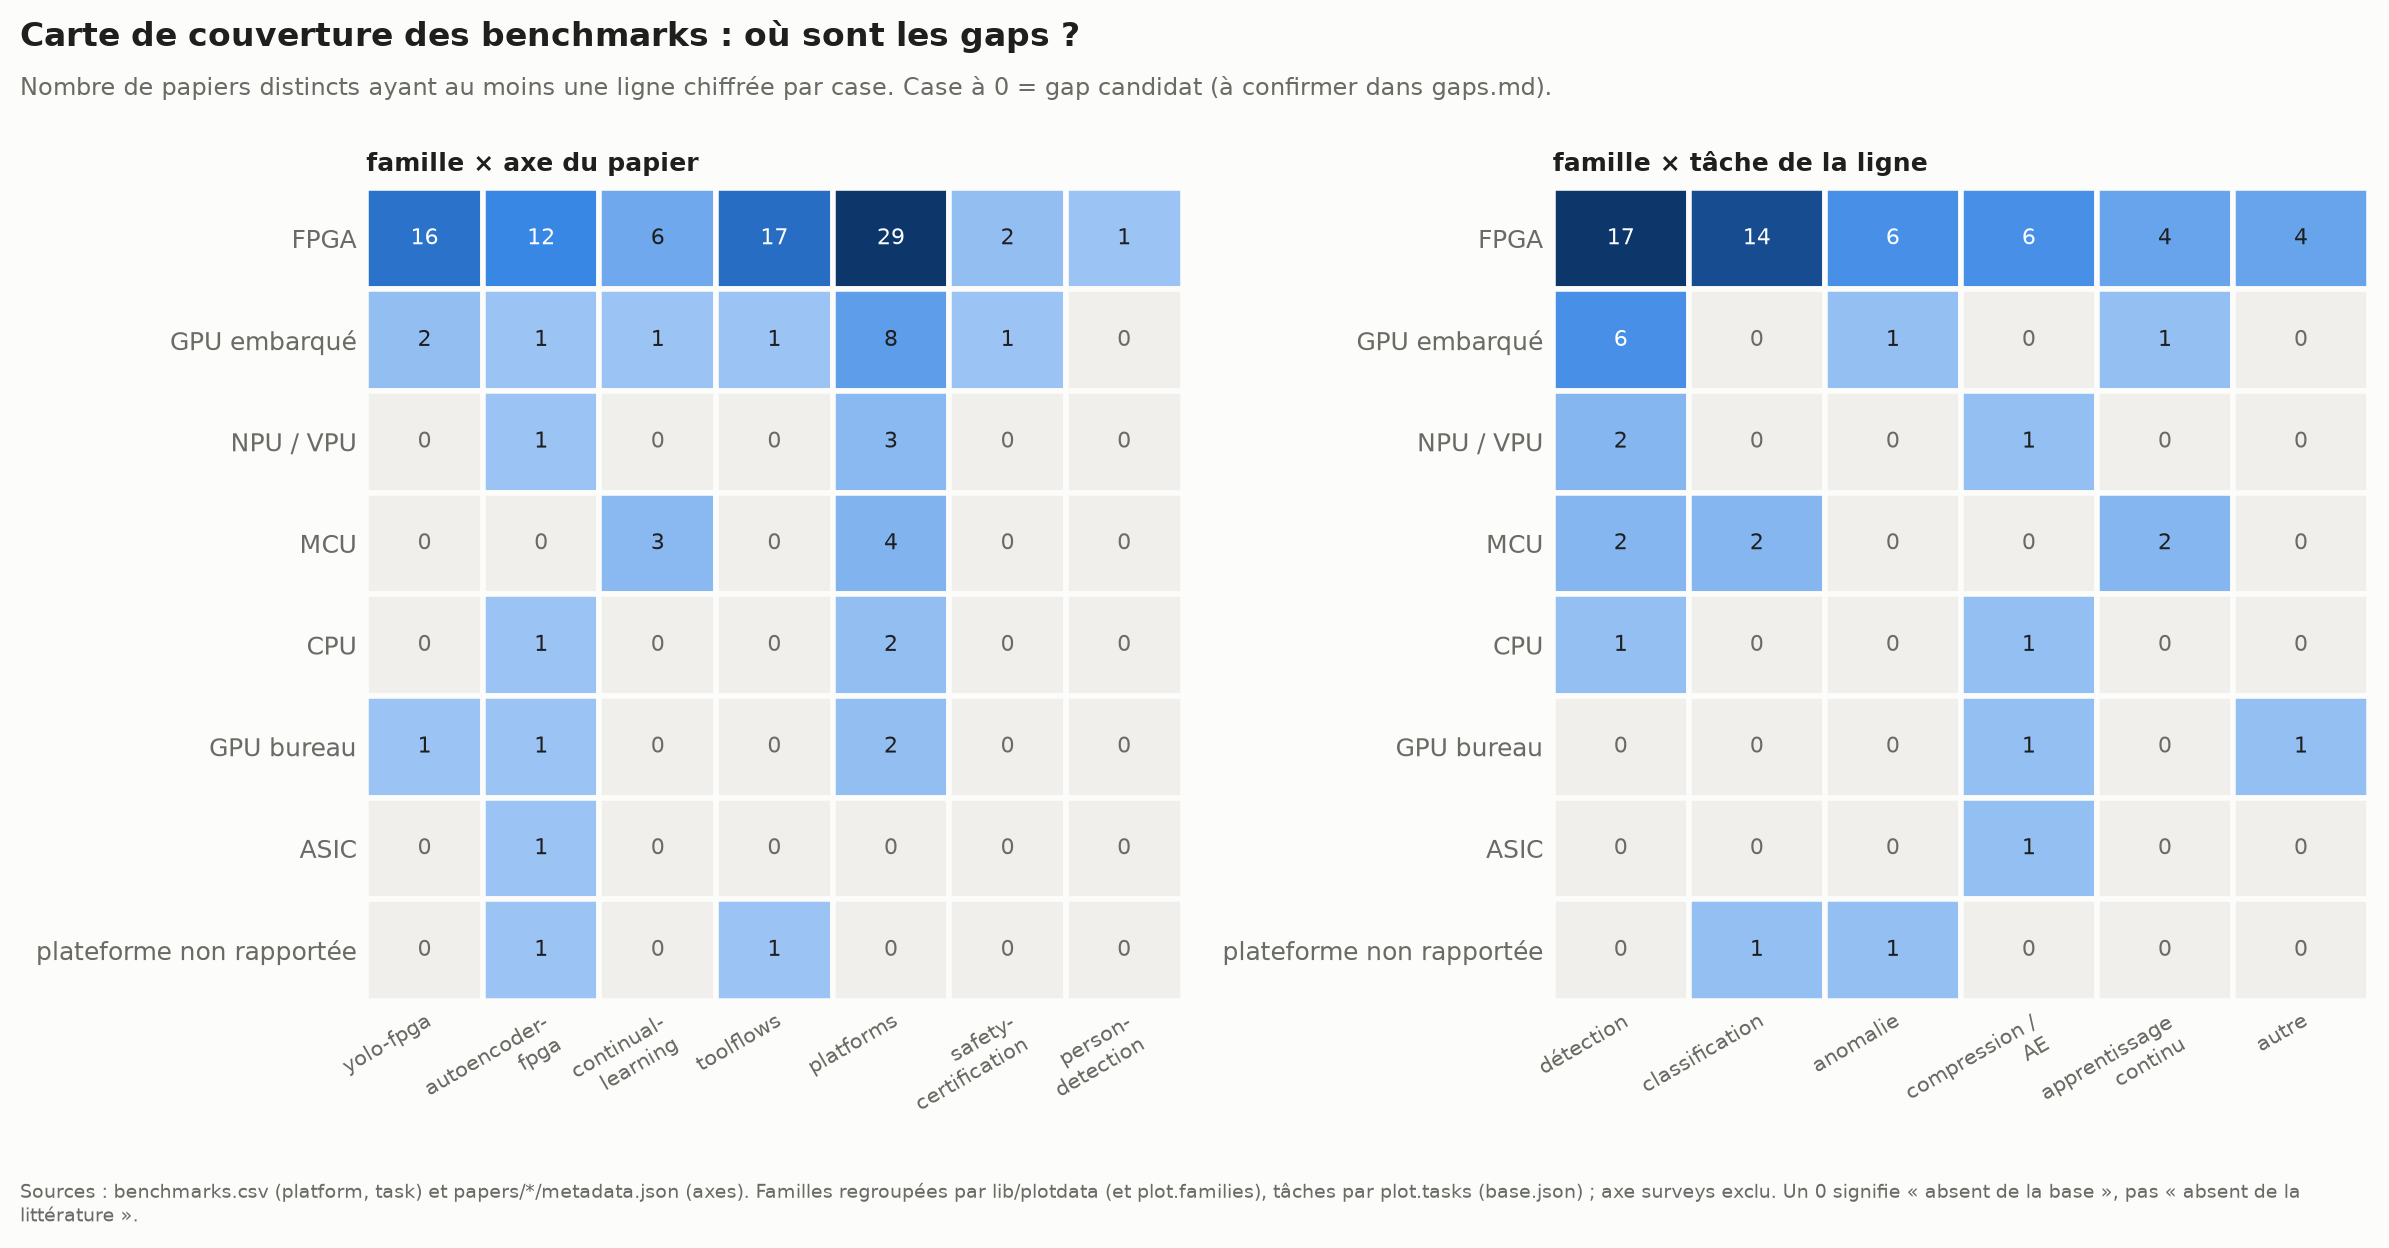
\includegraphics[width=0.8\linewidth]{fig/corpus_gaps.png}

  \raggedright\scriptsize
  Colonnes \emph{safety-certification} et \emph{person-detection} : 2 et 1 papiers FPGA avec
  au moins une ligne chiffrée. Un 0 signifie « absent de la base ».
\end{frame}

\begin{frame}{Annexe : incertitude en détection, et mitigations peu coûteuses}
  \footnotesize
  \textbf{Incertitude en détection} (Feng 2020, RetinaNet)
  \begin{itemize}
    \item la mAP ne mesure pas la qualité de l'incertitude ;
    \item modéliser directement la variance est essentiel ; MC-Dropout ou ensembles trop
          coûteux (2 à 3 FPS pour 10 passes) ;
    \item sous décalage de domaine (Lyft), la mAP tombe vers 5 à 6 pour toutes les variantes.
  \end{itemize}

  \textbf{Mitigations recensées par Rech 2024} (§VI, chiffres d'autres travaux, non
  comparables entre eux)
  \begin{itemize}
    \item ABFT : jusqu'à 85\,\% des erreurs critiques détectées ;
    \item cohérence temporelle entre images : $\approx$\,70\,\% ;
    \item RP-DWC : 75\,\% pour moins de 20\,\% de surcoût.
  \end{itemize}
  \textbf{Évaluation de la résilience} (Ruospo 2023) : simulation RTL d'un petit CNN
  $\approx$\,25 min par inférence ; résultats d'injection variables selon le composant et la
  température.
\end{frame}

\begin{frame}{Annexe : glossaire}
  \footnotesize
  \begin{tabularx}{\textwidth}{@{}p{2.2cm} L@{}}
    \toprule
    SIL / PL & niveaux d'intégrité de sécurité (IEC 61508 / 62061) et de performance
      (ISO 13849), définis par une probabilité de défaillance dangereuse par heure \\
    DAL & niveau d'assurance du développement en aéronautique \\
    FIT & défaillances par $10^9$ heures de fonctionnement \\
    SEU & inversion d'un bit par une particule (mémoire de configuration, BRAM, registres) \\
    TMR & triplication avec vote majoritaire \\
    ODD & domaine opérationnel de conception : conditions dans lesquelles le système est
      censé fonctionner \\
    OOD & entrée hors de la distribution d'entraînement \\
    FPPI & fausses détections par image ; « rappel à 0,1 FPPI » = rappel à fausse alarme fixée \\
    PTQ / QAT & quantification après entraînement / pendant l'entraînement \\
    DPU & moteur d'inférence programmable d'AMD-Xilinx (Vitis AI) \\
    Dataflow & un circuit dédié par couche, en pipeline (FINN, hls4ml, SATAY) \\
    \bottomrule
  \end{tabularx}
\end{frame}

\begin{frame}[allowframebreaks]{Références principales}
  \scriptsize
  \begin{itemize}
    \item Andéol et al., 2023. \textit{Confident Object Detection via Conformal Prediction
          and Conformal Risk Control: an Application to Railway Signaling}. arXiv:2304.06052\pre.
    \item Ashmore et al., 2019. \textit{Assuring the Machine Learning Lifecycle: Desiderata,
          Methods, and Challenges}. arXiv:1905.04223\pre.
    \item Aslansefat et al., 2020. \textit{SafeML: Safety Monitoring of Machine Learning
          Classifiers through Statistical Difference Measure}. arXiv:2005.13166\pre.
    \item Belcaid et al., 2024. \textit{Certified ML Object Detection for Surveillance
          Missions}. ERTS 2024. arXiv:2406.12362.
    \item Cheng et al., 2018. \textit{Runtime Monitoring Neuron Activation Patterns}.
          arXiv:1809.06573\pre.
    \item Choi et al., 2019. \textit{Gaussian YOLOv3}. arXiv:1904.04620.
    \item De Albuquerque Silva et al., 2022. \textit{ACETONE: Predictable Programming
          Framework for ML Applications in Safety-Critical Systems}. ECRTS 2022.
    \item Delseny et al., 2021. \textit{White Paper Machine Learning in Certified Systems}
          (DEEL). arXiv:2103.10529.
    \item EASA, 2020 / 2024. \textit{Concepts of Design Assurance for Neural Networks}
          (CoDANN I et II).
    \item EASA, 2024. \textit{Concept Paper: Guidance for Level 1 \& 2 Machine Learning
          Applications}, Issue 02.
    \item Fata et al., 2026. \textit{Low-Cost FPGA-Enhanced CNN Accelerator for Real-Time
          YOLO Object Detection and Classification}. IEEE Access 14.
    \item Feng et al., 2020. \textit{A Review and Comparative Study on Probabilistic Object
          Detection in Autonomous Driving}. IEEE T-ITS. doi:10.1109/TITS.2021.3096854.
    \item Gambardella et al., 2019. \textit{Efficient Error-Tolerant Quantized Neural Network
          Accelerators}. IEEE DFT.
    \item Gutierrez et al., 2026. \textit{NPU Accelerator: Quantized Real-Time Vehicle
          Detection on PYNQ-Z1 Using FINN}. arXiv:2609.24757\pre.
    \item Halme et al., 2018. \textit{Review of Vision-Based Safety Systems for Human-Robot
          Collaboration}. Procedia CIRP 72. doi:10.1016/j.procir.2018.03.043.
    \item Hawkins et al., 2021. \textit{Guidance on the Assurance of Machine Learning in
          Autonomous Systems (AMLAS)}. arXiv:2102.01564.
    \item Hendrycks, Gimpel, 2017. \textit{A Baseline for Detecting Misclassified and
          Out-of-Distribution Examples in Neural Networks}. ICLR 2017.
    \item Henzinger et al., 2020. \textit{Outside the Box: Abstraction-Based Monitoring of
          Neural Networks}. arXiv:1911.09032, ECAI 2020.
    \item Henzinger et al., 2021. \textit{Scalable Verification of Quantized Neural
          Networks}. AAAI 2021.
    \item Huang et al., 2018. \textit{A Survey of Safety and Trustworthiness of Deep Neural
          Networks}. arXiv:1812.08342\pre.
    \item Karki et al., 2026. \textit{No Attention, No Problem: DPU-Aware Attention
          Approximation in Modern YOLO on FPGA}. arXiv:2607.13106\pre.
    \item Katz et al., 2017. \textit{Reluplex: An Efficient SMT Solver for Verifying Deep
          Neural Networks}. arXiv:1702.01135.
    \item Li et al., 2017. \textit{Understanding Error Propagation in Deep Learning Neural
          Network (DNN) Accelerators and Applications}. SC'17.
          doi:10.1145/3126908.3126964.
    \item Libano et al., 2019. \textit{Selective Hardening for Neural Networks in FPGAs}.
          IEEE TNS 66(1).
    \item Libano et al., 2020. \textit{Understanding the Impact of Quantization, Accuracy,
          and Radiation on the Reliability of CNNs on FPGAs}. IEEE TNS 67(7).
    \item Montgomerie-Corcoran et al., 2023. \textit{SATAY: A Streaming Architecture Toolflow
          for Accelerating YOLO Models on FPGA Devices}. ICFPT 2023.
    \item Narodytska et al., 2017. \textit{Verifying Properties of Binarized Deep Neural
          Networks}. arXiv:1709.06662.
    \item Rech, 2024. \textit{Artificial Neural Networks for Space and Safety-Critical
          Applications: Reliability Issues and Potential Solutions}. IEEE TNS 71(4).
    \item Rey et al., 2025. \textit{A Performance Analysis of YOLO Models for Deployment on
          Constrained Computational Edge Devices in Drone Applications}. Electronics 14(3).
    \item Ruospo et al., 2023. \textit{A Survey on Deep Learning Resilience Assessment
          Methodologies}. IEEE Computer 56(2). doi:10.1109/MC.2022.3217841.
    \item Salay et al., 2017. \textit{An Analysis of ISO 26262: Using Machine Learning Safely
          in Automotive Software}. arXiv:1709.02435\pre.
    \item Schlosser et al., 2023. \textit{A Framework for Benchmarking Real-Time Embedded
          Object Detection}. DAGM GCPR 2022, LNCS 13485.
    \item Shao et al., 2018. \textit{CrowdHuman: A Benchmark for Detecting Human in a Crowd}.
          arXiv:1805.00123.
    \item Thys et al., 2019. \textit{Fooling Automated Surveillance Cameras: Adversarial
          Patches to Attack Person Detection}. arXiv:1904.08653.
    \item Zhang et al., 2024. \textit{End-to-End Acceleration of the YOLO Object Detection
          Framework on FPGA-Only Devices}. Neural Computing and Applications 36(3).
  \end{itemize}
\end{frame}

\end{document}
